\documentclass{article}

\usepackage[margin = 1 in]{geometry}

\usepackage{graphicx, amsmath}
\graphicspath{ {./images/} }

\title{Ch. 10 Solutions}
\author{Principles of Microeconomics}
\date{\today}

\begin{document}

\maketitle

\section*{Quick Quiz}

\begin{enumerate}

\item (c) -- Dev's newly cut lawn has a positive impact on his neighbors even though Dev isn't compensated for that positive impact. 

\item (b) -- The social cost curve is above the supply curve because there are external costs on top of the private costs that the supply curve plots. The socially optimal quantity is less than the market quantity because buyers and sellers have no incentive to account for the external costs to bystanders. As a result, they trade the good more than is socially optimal. 

\item (a) --

	\begin{center}
	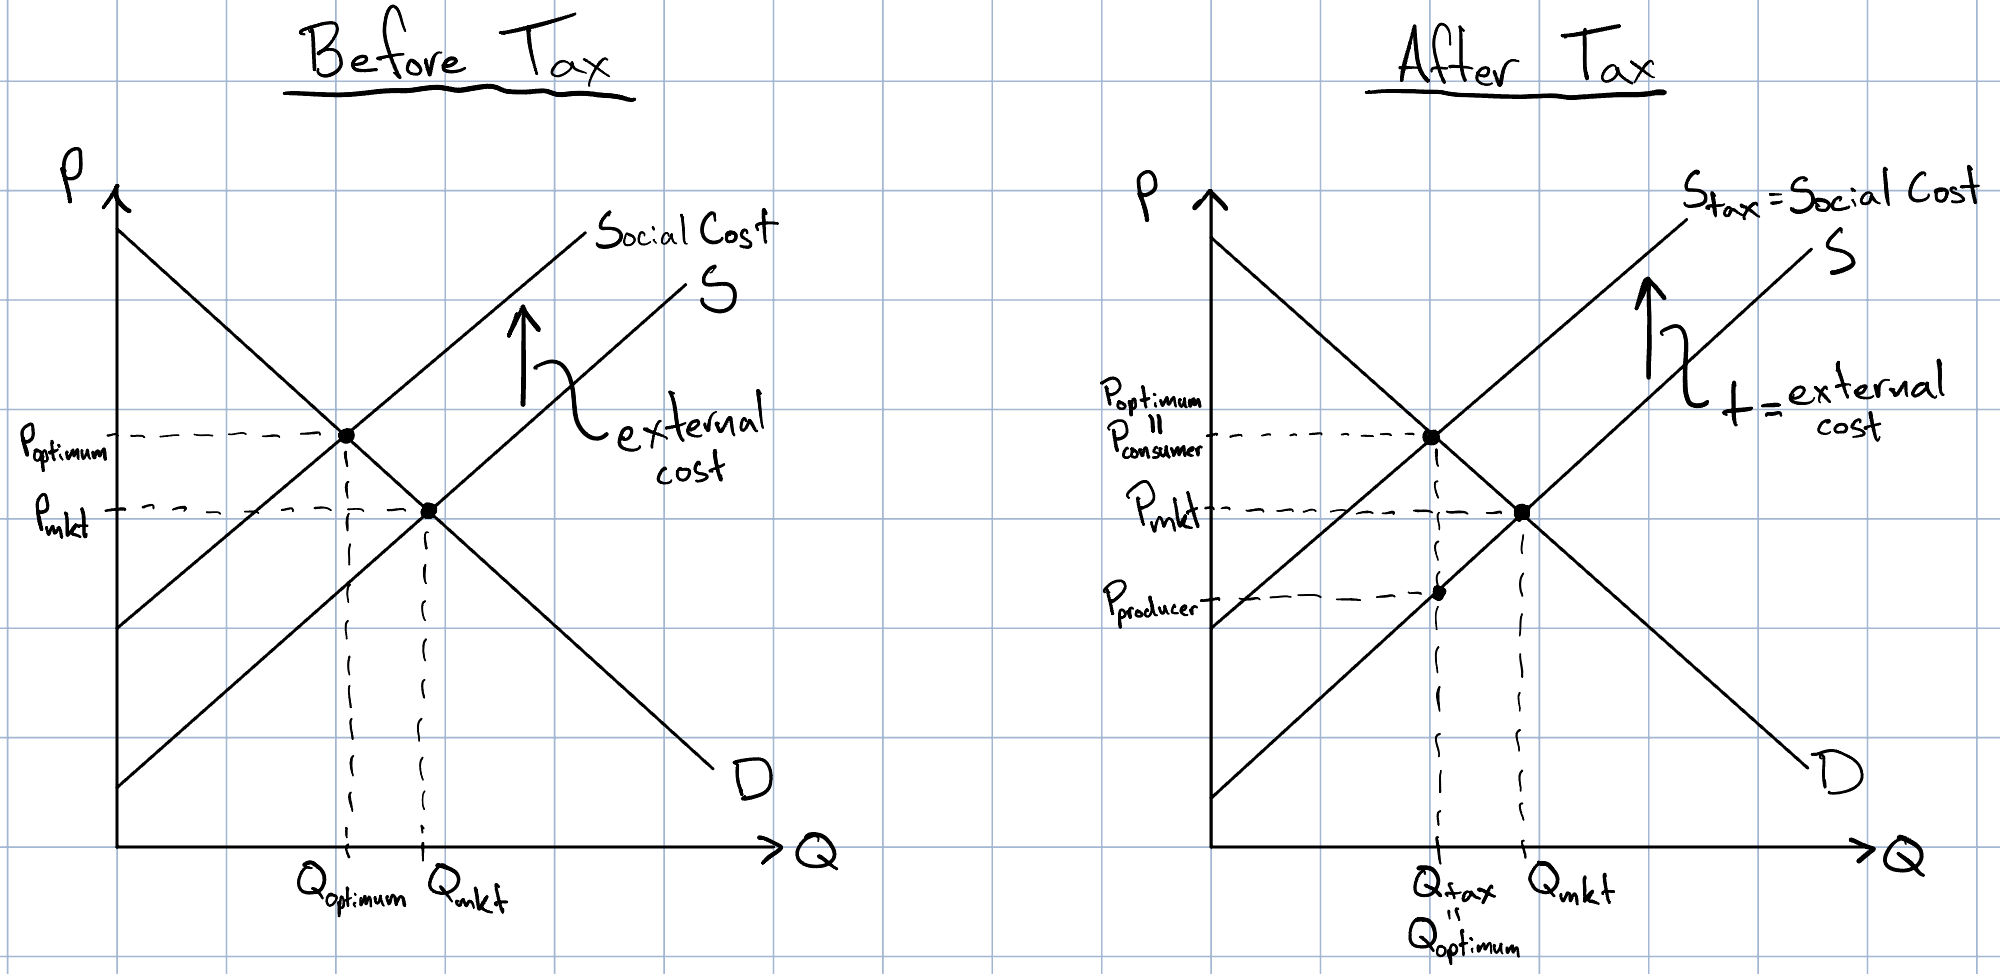
\includegraphics[width = 0.6\textwidth]{ch10_qq3}
	\end{center}

\item (d) -- Corrective taxes make markets more efficient. That means they increase total surplus and therefore decrease deadweight loss.

\item (b) --

	\begin{align*}
	Tax \ Revenue &= Q_{tax} \cdot t \\
	Q_{tax} &= Q_{permits} \\
	Q_{tax} &= 500 \\
	\implies \$25,000 &= 500 \cdot t \\
	50 &= t
	\end{align*}
	
\item (c) -- Otherwise, a corrective tax is a more efficient solution. It allows the firms that can reduce pollution at a low cost to reduce more and the firms that can only reduce pollution at a high cost to reduce less. 

\item (a) -- This is true as long as the actors can negotiate incurring prohibitive costs. 

\item (c) -- The parties must be able to negotiate for the Coase Theorem to apply.

\end{enumerate}

\section*{Questions for Review}

\begin{enumerate}

\item Carbon emissions are a negative externality of electricity consumption. Healthier neighbors are a positive externality of vaccination.

\item If a firm's production process has a negative externality, that means there's an external cost to production in addition to the private cost to producers. As a result, the social cost of production is higher than the private cost of production, so the social cost curve is higher than the supply curve. The optimal quantity is the intersection of demand and social cost, the quantity where the benefit to consumers equals the cost to society.
	\begin{center}
	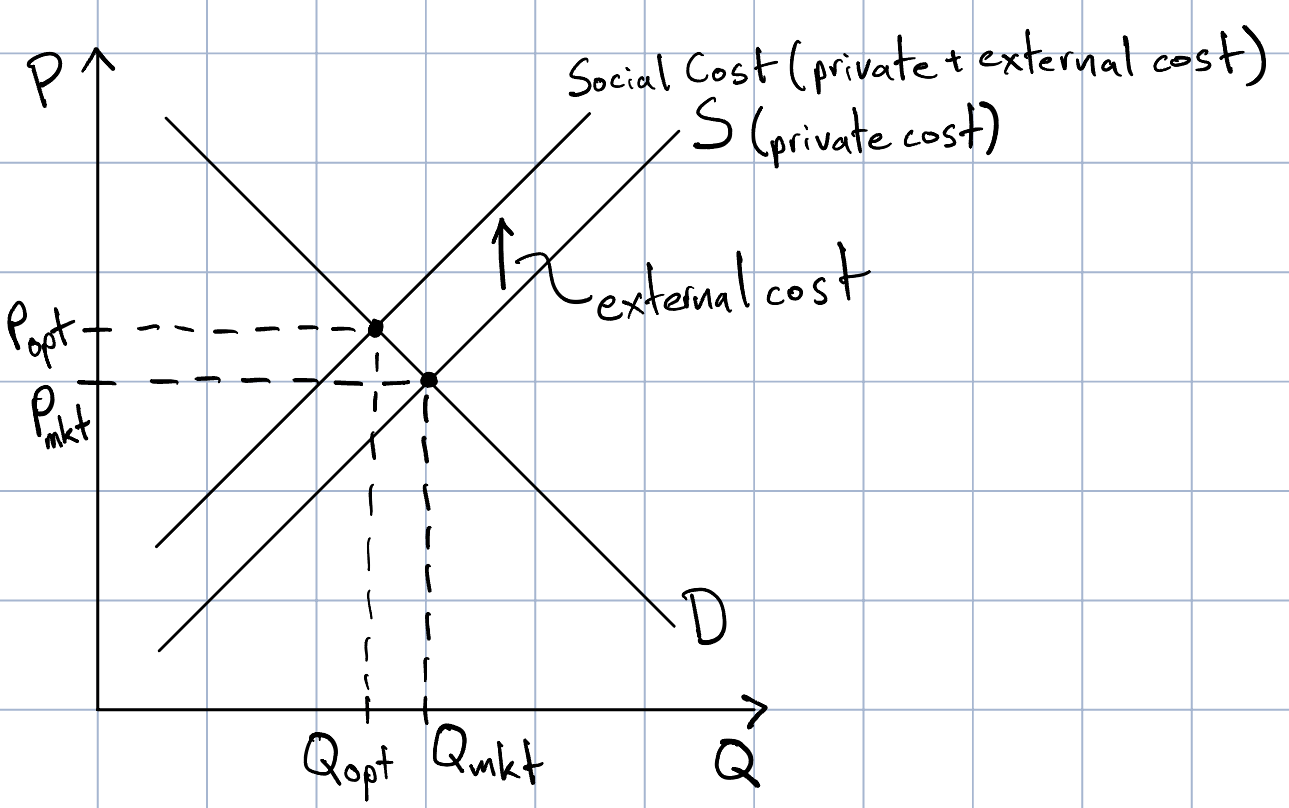
\includegraphics[width = 0.5\textwidth]{ch10_qfr2}
	\end{center}
	
\item When firms do research, their discoveries can create positive technological spillovers for other firms. In other words, other firms can benefit from the knowledge the research creates. As a result, research has a positive externality, so the optimal quantity of research is greater than the research that firms would do in an unregulated market. Patents attempt to internalize the externality by giving firms property rights over their discoveries. That way, other firms can't take advantage of the discoveries without paying the discoverers. 

\item Private negotiation, social norms, and charity are all potential non-governmental solutions.

\item According to the Coase theorem, the outcome depends on two things -- how much I value a smoke-free room relative to how much they value smoking inside and how easy it is for us to negotiate. If we can negotiate with sufficiently little cost, we should be able to reach a resolution. If my roommate values smoking more than I value a smoke-free room, we will negotiate a solution that allows them to keep smoking. If my roommate values smoking less than I value a smoke-free room, we will negotiate a solution that prohibits them from smoking. In both scenarios, the outcome is efficient.

\end{enumerate}

\section*{Problems and Applications}

\begin{enumerate}

\item The steering wheel lock has a negative externality on other car owners. If a car thief sees that one person's car has the steering wheel lock, then they're more likely to steal another person's car. The tracking system has a positive externality on other car owners. If a car thief steals a car with the tracking system, they are more likely to get caught which makes them less likely to steal anyone else's car in the future. 

One possible policy implication is that the government should place a corrective tax on steering wheel locks and subsidize tracking systems.

\item

	\begin{enumerate}
	
	\item Fire extinguishers prevent fires from spreading. The more fire extinguishers a building has, the less likely a fire is to spread to other buildings. That benefits the owners of other buildings. 
	
	\item \phantom{x}
	
		\begin{center}
		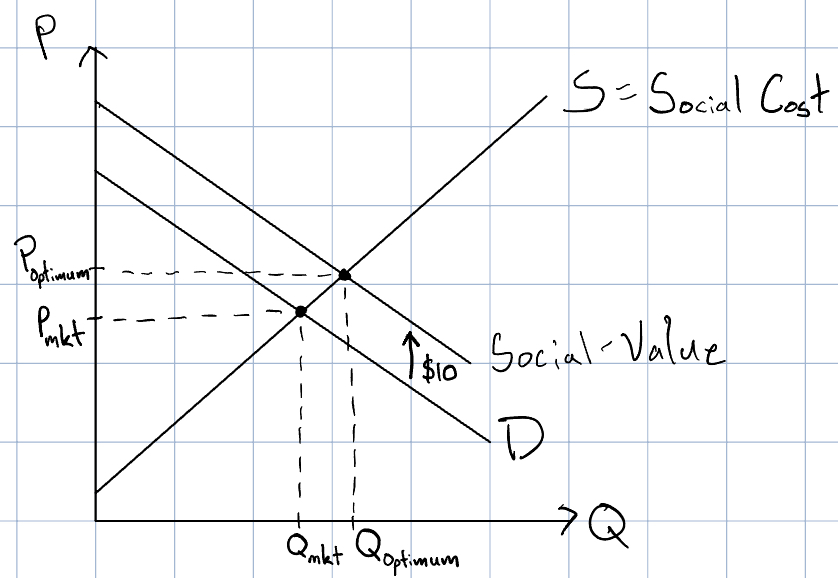
\includegraphics[width = 0.3\textwidth]{ch10_paa2b}
		\end{center}
		
	\item See the diagram above. Consumers choose to purchase the number of fire extinguishers that is best for them. They don't factor in the benefits to their neighbors. As a result, they consume less than the societally optimal amount. 
	
	\item The government could put a \$10 per unit subsidy on fire extinguisher consumption. That way, consumers' private value for fire extinguishers would equal the social value.
	
	\end{enumerate}
	
\item

	\begin{enumerate}
	
	\item \phantom{x}
	
		\begin{center}
		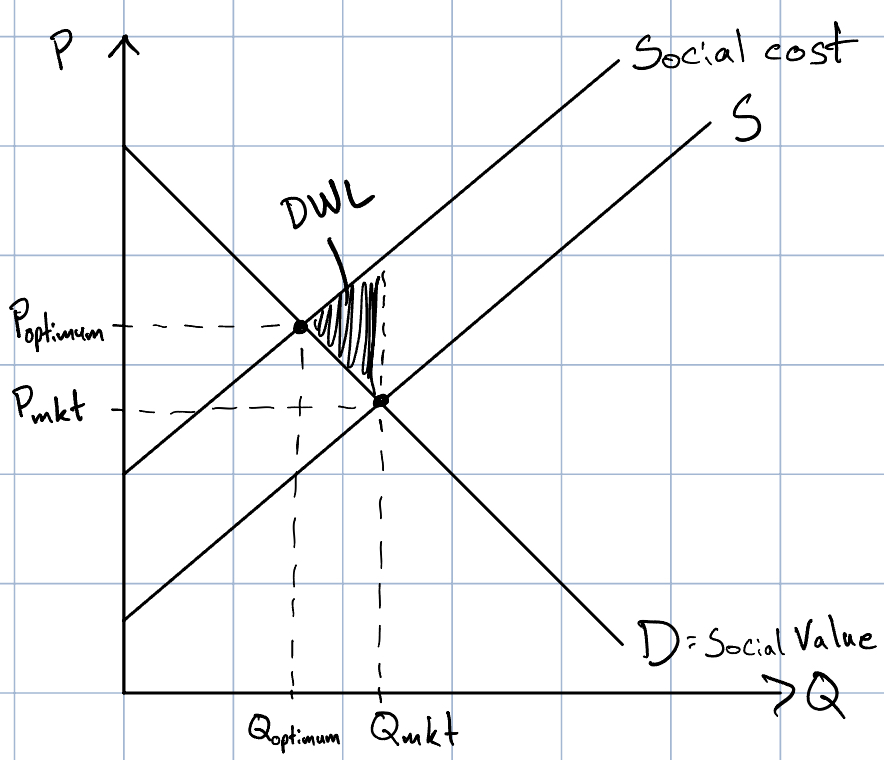
\includegraphics[width = 0.3\textwidth]{ch10_paa3a}
		\end{center}
	
	\item After quantity surpasses $Q_{Optimum}$, the social cost of alcohol exceeds the social value. Therefore, every unit sold beyond $Q_{Optimum}$ generates deadweight loss. The shaded region is the total deadweight loss.
	
	\end{enumerate}
	
\item 

	\begin{enumerate}

	\item To reduce pollution efficiently, we have to do it in the lowest cost way. It's possible that some firms can reduce pollution at lower costs than others. If that's the case, the lowest cost way to reduce pollution would be for those firms to reduce their pollution more, and the other firms to reduce their pollution less.
	
	\item If the command-and-control approach mandates a uniform reduction, then all firms are reducing by the same amount or to the same level. That means firms with lower reduction costs aren't necessarily reducing their pollution more and firms with higher reduction costs aren't necessarily reducing their pollution less. 
	
	\item Corrective taxes and tradable pollution permits force firms to pay for each unit of pollution they create. Firms that can reduce pollution at a lower cost will reduce their pollution substantially to avoid paying the tax or buying permits. Firms that can only reduce pollution at a high cost will reduce their pollution less and pay more tax or buy more permits.

	\end{enumerate}
	
\item

	\begin{enumerate}
	
	\item Each Whovillian will consume four bottles because their willingness to pay is only greater than \$1.50 for the first four bottles. Their consumer surplus is
		\[ CS = 5 - 1.5 + 4 - 1.5 + 3 - 1.5 + 2 - 1.5 = 8. \]
		
	\item The social cost of each bottle is now \$2.50. That means total surplus per person is 
		\[TS = 5 - 2.5 + 4 - 2.5 + 3 - 2.5 + 2 - 2.5 = 4. \]
		
	\item The welfare that Cindy generates increases to 
		\[ TS = 5 - 2.5 + 4 - 2.5 + 3 - 2.5 = 4.5. \]
		As a result, total surplus in Whoville increases by 0.5.
		
	\item Now the private cost of each bottle is \$2.50. That means each Whovillian will only consume three bottles. 
		\begin{align*}
		CS &= 5 - 2.5 + 4 - 2.5 + 3 - 2.5 = 4.5 \\
		External \ Cost &= 3(1) = 3 \\
		Government \ Revenue &= 3(1) = 3 \\
		TS &= CS - External \ Cost + Gov't \ Revenue \\
		&= 4.5 - 3 + 3 = 4.5
		\end{align*}
		
	\item I would support the mayor's policy. It increases total surplus per person.
	
	\end{enumerate}
	
\item

	\begin{enumerate}
	
	\item Bruno's loud rock creates a negative externality because Placido can probably hear it through the wall, and she dislikes rock.
	
	\item The land lord could ban loud music. That policy could lead to an inefficient outcome though because the loud music might create a bigger benefit for Bruno than it creates a cost for Placido.
	
	\item Placido could offer to pay Bruno to turn down his music. If Placido's costs from hearing the rock are greater than Bruno's benefits, she would eventually offer him a price that exceeds his benefits, and he would turn down his music. When her costs exceed his benefits, that's the efficient outcome. If Placido's costs are less than Bruno's benefits she would never offer him a price that exceeds his benefits, and he would continue playing his music at high volume. When his benefits exceed her costs, that's the efficient outcome.
	
	If there are transaction costs to their negotiation, they might not reach the efficient outcome. For example, they might not speak the same language, or they may detest each other from some prior dispute. In both cases, negotiating becomes onerous, so they might not reach an agreement.
	
	\end{enumerate}
	
\item

	\begin{enumerate}
	
	\item \phantom{x}
	
		\begin{center}
		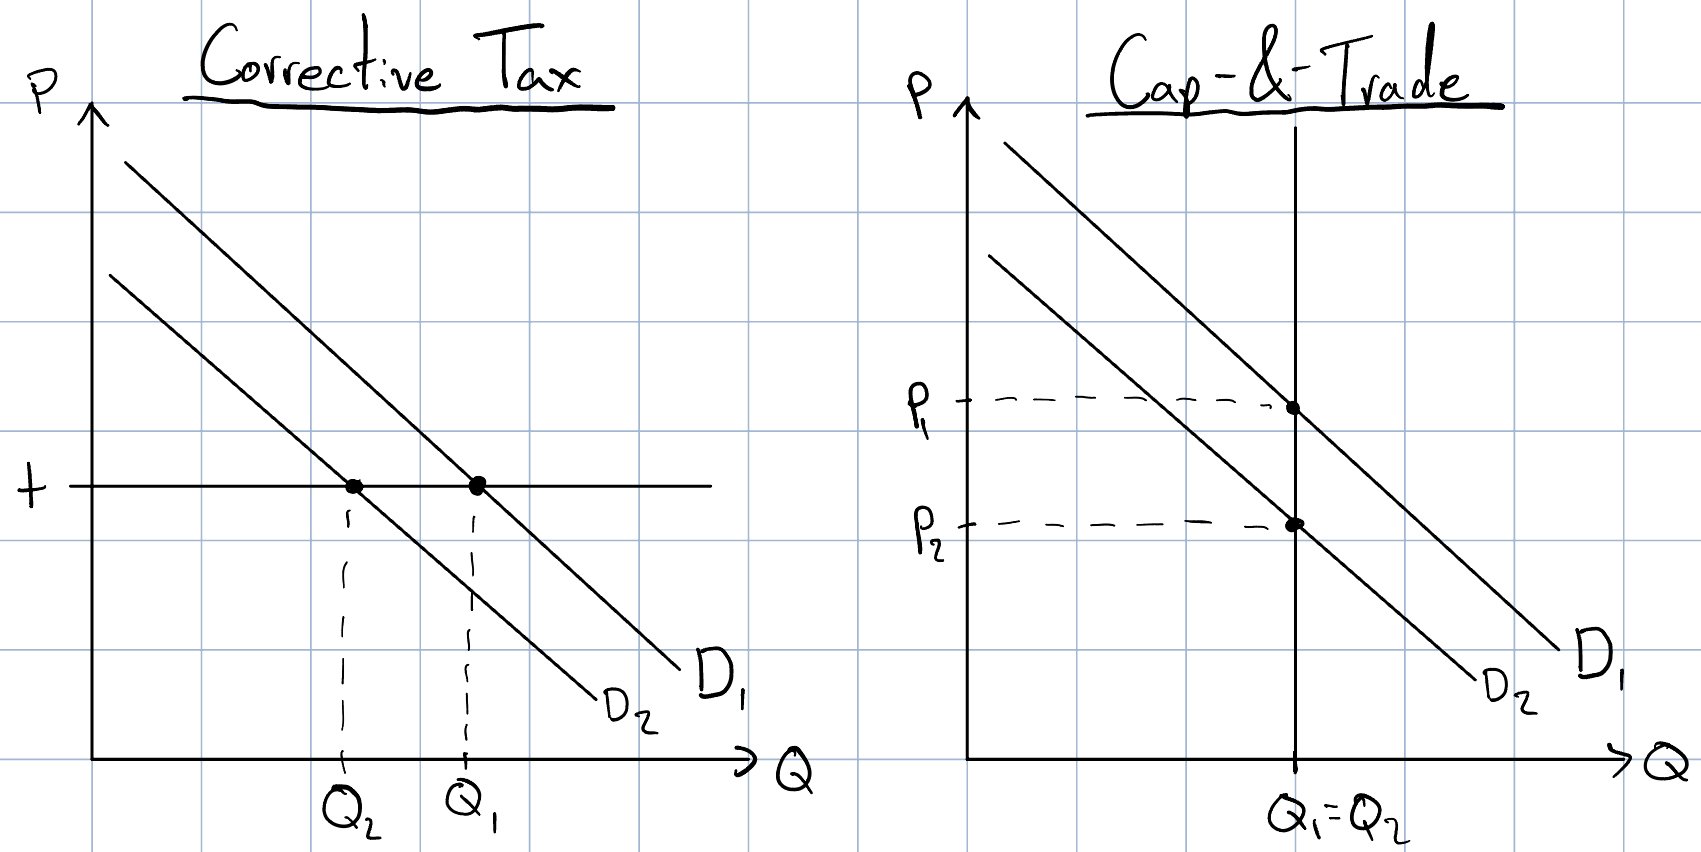
\includegraphics[width = 0.6\textwidth]{ch10_paa7a}
		\end{center}
		
	\item The improvement in technology for controlling pollution will decrease the demand for pollution. Under the corrective tax, the price of polluting remains constant at the level of the tax, but the quantity of pollution goes down. Under the cap-and-trade policy, the quantity of pollution will remain fixed at the capped amount, but the price of polluting will go down because the permits will be less valuable.
	
	\end{enumerate}
	
\item

	\begin{enumerate}
	
	\item It does not. Under an auction system, the firms that value polluting the most will win the permits. Under a distribution system, the permits are tradable, so the firms that value polluting more will buy the permits from firms who value polluting less. The firms who value polluting more will be the firms who face higher costs for reducing their pollution. Therefore, under both systems, we get the efficient outcome because the firms who face higher costs will reduce their pollution less and the firms who face lower costs will reduce their pollution more.
	
	\item It does not. The firms who value them more will buy them from the firms who value them less. As a result, the firms who face high costs for reducing their pollution will reduce less, and the firms who face low costs will reduce more. 
	
	\end{enumerate}
	
\item 	

	\begin{enumerate}
	
	\item The value each firm places on a permit is equal to the cost the permit saves them by allowing them to pollute. That means Firm B values them the most and C the least. Firm B buys all of Firm C's permits for some price between \$10 and \$30 because Firm B is willing to pay more than the \$10 value that Firm C places on the permits. After buying 20 permits, Firm B can continue to produce its original 40 units of pollution, so it doesn't buy any more from Firm A. As a result, Firm A keeps its 20 permits. 

Since Firm C ends up with no permits, they spend $20 \cdot \$10 = \$200$ reducing their pollution. Since Firm A ends up with 20, they spend $10 \cdot \$20 = \$200$ reducing their pollution. Since Firm B ends up with 40 permits, they don't reduce their pollution. That means the total cost is \$400.

	\item Firm A would have spent $10 \cdot \$20 = \$200$ reducing their pollution. Firm B would have spent $20 \cdot \$30 = \$600$ reducing their pollution. Firm C would have spent \$0 reducing their pollution because they would have enough permits to cover their pollution. That means the total cost would be \$800.

	\end{enumerate}

\end{enumerate}

\end{document}